% !TEX root = diplomarbeit.tex
\chapter{Firmware}
\renewcommand{\kapitelautor}{Autor: Christina Bornberg, Lucas Ullrich}

%%%%%%%%%%%%%%%%%%%%%%%%%%%%%%%%%%%%%%%%%%%%%%%%%%%%%%%%%%%%%%%%%%%%%%%%%%%%%%%
\section{Allgemeine technische Planung}

  \subsection{Tischkonzept}

  \subsection{Flussdiagramme}
  Für einen besseren Überblick über die einzelnen Programme und deren geforderten Funktionen wurden einzelne Flussdiagramme des gesamten Prozesses erstellt.
  Diese dienen nachfolgend als Orientierung beim Programmieren der einzelnen Funktionen.

  \begin{figure}[tbh]
    \begin{centering}
      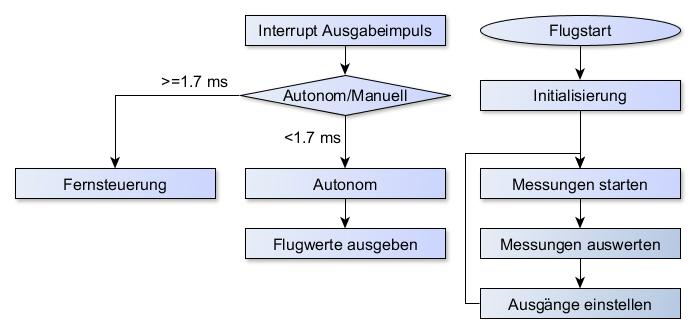
\includegraphics[width = \textwidth]{Bilder/Flussdiagramm}
    \par\end{centering}
    \caption{Flussdiagramm des Gesamtablaufs}
    \label{Flussdiragramm}
  \end{figure}

  Für die weiteren Programmteile wurden jeweils noch detailliertere Flussdiagramme erstellt.

  \subsection{Tools}

    \subsubsection{GitHub}


    \subsubsection{MPLAB}

%%%%%%%%%%%%%%%%%%%%%%%%%%%%%%%%%%%%%%%%%%%%%%%%%%%%%%%%%%%%%%%%%%%%%%%%%%%%%%%
\section{Navigation}

  \subsection{Technische Planung}

  \subsection{Umsetzung}

    \subsubsection{Vergleichen der Frames}
    Für den Vergleich des aktuellen mit dem letzten Frame, werden zwei \glslink{Struktur}{Strukturen} verwendet, die über folgende Mitglieder verfügt.
    \begin{itemize}
      \item \textbf{num}\\
      ist die ID des getrackten Colorcodes, er besteht aus einer zweistelligen Zahl.
      \item \textbf{pos\_x}\\
      ist die X-Position des Colorcodes. Der Wert bezieht sich auf das Zentrum des Objektes.
      \item \textbf{pos\_y}\\
      ist die Y-Position des Colorcodes. Der Wert bezieht sich auf das Zentrum des Objektes.
      \item \textbf{height}\\
      ist die, vom Ultraschall übergebene Höhe.
      \item \textbf{angle}\\
      ist die Rotation des Colorcodes. Da er zweifarbig ist, kann die PIXY CMUcam5 die Rotation des Objektes feststellen.
    \end{itemize}

    Quelle: \textcolor{red}{TITEL FEHLT \cite{Structs}, das sollte verlegt werden -Lucas}

    Zuerst wird die ID des Colorcodes verglichen, um herauszufinden, ob das Farbobjekt das selbe wie im letzten Frame ist.
    Sollte dies der Fall sein, werden die Koordinaten x und y und die Rotation mit den Werten der älteren Struktur verglichen und gespeichert.
    Diese werden bei den folgenden Funktionen verwendet, um zu überprüfen, ob der Hexacopter die richtige Geschwindigkeit hat.

    \subsubsection{Aileron, Elevator und Rudder anhand der Kameradaten}
    Durch die PIXY CMUcam5 kann die Position des Hexacopters, relativ zu einem Colorcode, festgestellt werden. Gegebenenfalls werden anschließend die Flugparameter verändert.

    \begin{figure} [tbh]
      \begin{centering}
        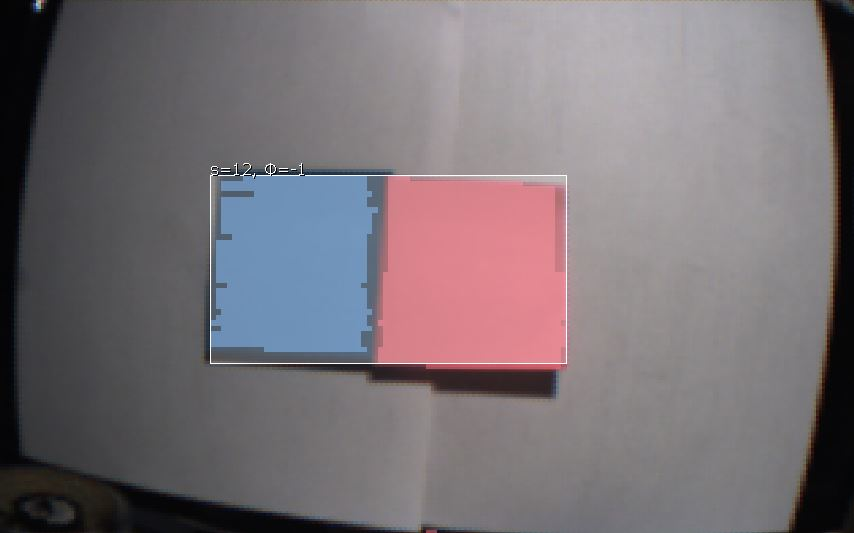
\includegraphics[width = \textwidth]{Bilder/Farbcode_erkannt}
      \par\end{centering}
      \caption{Ein erkannter Farbcode}
      \label{Farbcode_erkannt}
    \end{figure}
    Die Position wird anhand solcher Farbcodes erkannt, im Tischkonzept ist hinterlegt in welcher Reihenfolge der Hexacopter die Farbcodes suchen muss.
    Er fliegt anschließend so lange, bis er über dem aktuellen Farbcode ist, dieser also mittig im Bild ist und sucht darauf den nächsten.


    Die PIXY CMUcam5 XXXXXX % IRGENDWAS MIT X diese länge, y diese länge; %



      \begin{itemize}
        \item \textbf{Überprüfen von Aileron}\\
        Die Überprüfung von Aileron bezieht sich auf die Beschleunigung nach Links und Rechts, was der x-Koordinate entspricht.

        Ziel der Funktion ist es, den Farbcode in die Mitte des Frames zu bekommen. Der Idealzustand befindet sich zwischen 150 und 170.
        Sollte dieser Zustand erreicht werden, bleibt der Wert von Aileron unverändert und der Hexacopter fliegt weiterhin mit einer unveränderten Beschleunigung an der
        x-Koordinate.
        Sollte dies nicht der Fall sein, muss der Wert auf einige Komponenten \textcolor{red}{XXXXX} überprüft werden.
        Wenn der Farbcode zu weit auf der rechten Seite liegt, das bedeutet, wenn der Wert des Mittelpunktes vom Farbobjekt höher als 170 ist,
        muss der Hexacopter nach rechts fliegen, um seine Position zu korrigieren.
        Dabei muss zuerst verglichen werden, ob sich der Hexacopter in die richtige Richtung bewegt. Sollte er in die falsche Richtung
        fliegen, wird der Aileron-Flugparameter gesenkt, dies setzt die Beschleunigung nach Rechts vorraus.
        Wenn die Beschleunigung nach rechts hoch genug ist und die Drohne tatsächlich nach rechts fliegt, wird die Geschwindigkeit überprüft.
        Die Geschwindigkeit wird durch die Differenz der x-Koordinate beider Strukturen herausgefunden. Die Einheit ist in diesem Fall

        \item \textbf{Überprüfen von Elevator}\\
        Position der Farbobjekte (CHECK AILERON \& ELEVATOR)
        Wenn ein Farbobjekt nicht im gewünschten Bereich plaziert ist, muss der Hexacopter weiter nach links oder weiter nach rechts fliegen.
        \item \textbf{Überprüfen von Rudder}\\
        Rotation der Farbojekte (CHECK RUDDER)
        Wenn der Hexacopter über einem Farbobjekt fliegt, soll er kontrollieren, ob der 2-Farbige Code die richtige Rotation hat und sich im richtigen Bereich des Bildschirmes befindet. Wenn diese Informationen richtig sind, darf der Copter zum nächsten Farbobjekt fliegen.
        Durch dieses System könne die genauen Wege vorgegeben werden und können sich durch das gesamte Restaurant verteilen. Durch die Rotation der Codes können auch Kurven eingebaut werden.

        Richtung (CHECK RUDDER)
        Durch die Rotation der Colorcodes, kann der Hexacopter bestimmen, ob er den richtigen Weg und in die richtige Richtung fliegt, wenn er am Weg zurück zur Base ist, muss er den umgekehrten Colorcode verwenden. (Rotation 180Grad)
      \end{itemize}

    \subsubsection{Throttle anhand des Ultraschallsensors}

    Starten und landen auf Landeplattformen (CHECK THROTTLE)
    Der Hexacopter startet und landet auf den mit ebenfalls mit Colorcodes gekennzeichneten Landeplattformen.
    Bei einem Fehler, besteht auch das Landen auf einem beliebigen Fleck

    Höhe korrigieren (CHECK THROTTLE)
    Höhenunterschied zwischen Tisch und Boden

    \subsubsection{Speichern der alten Daten}

    \subsubsection{Ausgabe der Steuersignal}
    Nachdem die Steuersignale berechnet und korrigiert wurden müssen diese an den Hexacopter ausgegeben werden. Dies muss periodisch alle $\SI{20}{\milli\second}$ geschehen.
    Der Flightcontroller erkennt jeweils die einzelnen Impulse und steuert die Rotoren entsprechend an.

    Diese Impulse werden Interrupt-gesteuert ausgegeben, der Interrupt wird von dem Gear-Pin erzeugt welcher gleichzeitig für den Flugmodus verantwortlich ist.

    \lstset{language = c}
    \begin{lstlisting}
interrupt void Isr() {
  if(CCP1IF == 1) {
    CCP1IF = 0;
    T1CONbits.TMR1ON = 0;
    SignalOut();
    NOP();
  }
  if(TMR3GIF == 1) {
    TMR3GIF = 0;
    ModeCheck();
    SignalOut();    /* initial call after remaining break to 20 ms
                     * starts with Aileron (needs to be set in last
                     * case statement, case 0) following delays will
                     * be processed by the previous routine */
    pulsecounter++;
  }
}

void SignalOut(void) {
  switch(pin_out) {
    case 'A': {
      A = 1;
      Delay(a_actors[0].aile);
      pin_out = 'E';
      break;
    }case 'E': {
      A = 0;
      E = 1;
      Delay(a_actors[0].elev);
      pin_out = 'T';
      break;
    }
    \end{lstlisting}
    Die weiteren Signale (Throttle und Rudder) werden auf die gleiche Weise ausgegeben.
    Die Delay-Funktion stellt die Compare-Einehit so ein, dass nach der gewünschten Pulsdauer des Ausgangs ein Interrupt hervorgerufen wird.

%%%%%%%%%%%%%%%%%%%%%%%%%%%%%%%%%%%%%%%%%%%%%%%%%%%%%%%%%%%%%%%%%%%%%%%%%%%%%%%
\section{Objekterkennung}

  \subsection{Technische Planung}

  \subsection{Umsetzung}

  \subsection{Herausforderungen und Lösungen}

%%%%%%%%%%%%%%%%%%%%%%%%%%%%%%%%%%%%%%%%%%%%%%%%%%%%%%%%%%%%%%%%%%%%%%%%%%%%%%%
\section{Sicherheit}

  \subsection{Technische Planung}

  \subsection{Umsetzung}

  \subsection{Herausforderungen und Lösungen}

%%%%%%%%%%%%%%%%%%%%%%%%%%%%%%%%%%%%%%%%%%%%%%%%%%%%%%%%%%%%%%%%%%%%%%%%%%%%%%%
\section{Systemausfall}

  \subsection{Technische Planung}

  \subsection{Umsetzung}

  \subsection{Herausforderungen und Lösungen}
